% This LaTeX document needs to be compiled with XeLaTeX.
\documentclass[10pt]{article}
\usepackage[a4paper, margin=0.8in]{geometry}
\usepackage[utf8]{inputenc}
\usepackage{amsmath}
\usepackage{amsfonts}
\usepackage{amssymb}
\usepackage[version=4]{mhchem}
\usepackage{stmaryrd}
\usepackage{graphicx}
\usepackage[export]{adjustbox}
\graphicspath{ {./images/} }
\usepackage[fallback]{xeCJK}
\usepackage{polyglossia}
\usepackage{fontspec}
\usepackage{setspace}
\usepackage{enumitem}

\newcommand{\sol}{\textbf{解:} }

\onehalfspacing

\allowdisplaybreaks
\setcounter{section}{5}
\setcounter{subsection}{1}
\begin{document}
\subsection{圆的标准方程式}
\subsection*{(选择题)}

\begin{enumerate}[leftmargin=*]
  \item 求以 $(6,7)$ 与 $(4,-3)$ 之连线为直径之圆的方程式。
  
  \sol{}
  
  半径为 $\dfrac{\sqrt{(6-4)^{2}+(7-(-3))^{2}}}{2}=\dfrac{\sqrt{2^{2}+10^{2}}}{2}=\dfrac{\sqrt{104}}{2}=\dfrac{2\sqrt{26}}{2}=\sqrt{26}$,
  
  圆心为 $\left(\dfrac{6+4}{2}, \dfrac{7+(-3)}{2}\right)=(5,2)$, 所以方程式为 $(x-5)^{2}+(y-2)^{2}=26$。\hfill$\blacksquare$
  
  \item 如果圆 $x^{2}+y^{2}=4^{2}$ 上的一点 $\mathrm{P}$ 到直线 $4 x+3 y-60=0$ 的距离是最小, 求 $\mathrm{P}$ 点的坐标。
  
  \sol{}
  \begin{flalign*}
    4x + 3y - 60 &= 0\\
    3y &= -4x + 60\\
    y &= -\dfrac{4}{3}x + 20\\
    m &= -\dfrac{4}{3}
  \end{flalign*}
  直线穿过圆心的法线方程为
  \begin{flalign*}
    y-0 &= \dfrac{3}{4}(x-0)\\
    y &= \dfrac{3}{4}x
  \end{flalign*}
  代入圆的方程得
  \begin{flalign*}
    x^{2} + \left(\dfrac{3}{4}x\right)^{2} &= 4^{2}\\
    x^{2} + \dfrac{9}{16}x^{2} &= 16\\
    \dfrac{25}{16}x^{2} &= 16\\
    x^2 &= \dfrac{256}{25}\\
    x &= \pm \dfrac{16}{5}
  \end{flalign*}
  当 $x = \dfrac{16}{5}$ 时, $y = \dfrac{12}{5}$, 当 $x = -\dfrac{16}{5}$ 时, $y = -\dfrac{12}{5}$。\hfill$\blacksquare$

  所以 $\mathrm{P}$ 点的坐标为 $\left(\dfrac{16}{5}, \dfrac{12}{5}\right)$。

  \item 求由圆 $(x-5)^{2}+(y-3)^{2}=9$ 上的一点到直线 $3 x+4 y=2$ 的最短距离。
  
  \sol{}
  
  直线 $3x+4y=2$ 与圆心 $(5,3)$ 的距离为 $\dfrac{|3(5)+4(3)-2|}{\sqrt{3^{2}+4^{2}}} = \dfrac{|15+12-2|}{5} = 5$。

  圆的半径为 $3$, 所以最短距离为 $5-3=2$。\hfill$\blacksquare$
  
  \newpage
  \item 点 $(5,3)$ 是圆 $(x-2)^{2}+(y+1)^{2}=25$ 的一直径的端点。求此直径另一端点的坐标。
  
  \sol{}

  设另一端点为 $(x, y)$, 已知圆心为 $(2, -1)$, 根据中点公式得
  \begin{flalign*}
    \dfrac{5+x}{2} &= 2\\
    5+x &= 4\\
    x &= -1\\
    \dfrac{3+y}{2} &= -1\\
    3+y &= -2\\
    y &= -5
  \end{flalign*}
  所以另一端点的坐标为 $(-1, -5)$。\hfill$\blacksquare$
\end{enumerate}

\section*{(作答题)}
\begin{enumerate}[leftmargin=*]
  \item 一正方形的四顶点 $\mathrm{A}, \mathrm{B}, \mathrm{C}, \mathrm{D}$ 顺序依反时针方向排列。若 $\mathrm{A}$ 点的座标为 $(1,3), \mathrm{BD}$落于直线 $2 x+y+5=0$ 上。试求出 $\mathrm{B}, \mathrm{C}, \mathrm{D}$ 三点的坐标。(不准用图解法。) 
  
  \sol{}

  直线 $2x+y+5=0$ 的斜率为 $-2$, 该直线过点 $(1,3)$ 的法线斜率为 $\dfrac{1}{2}$, 所以法线方程为
  \begin{flalign*}
    y-3 &= \dfrac{1}{2}(x-1)\\
    y &= \dfrac{1}{2}x - \dfrac{1}{2} + 3\\
    y &= \dfrac{1}{2}x + \dfrac{5}{2}
  \end{flalign*}
  代入直线方程得
  \begin{flalign*}
    2x + \dfrac{1}{2}x + \dfrac{5}{2} + 5 &= 0\\
    4x + x + 5 + 10 &= 0\\
    5x &= -15\\
    x &= -3\\
    y &= \dfrac{1}{2}(-3) + \dfrac{5}{2}\\
    &= 1
  \end{flalign*}
  所以正方形的中心为 $M(-3, 1)$。

  设 $\mathrm{B}$ 点和 $\mathrm{C}$ 点的坐标为 $(x, -2x-5)$。
  \begin{align*}
    \dfrac{AM}{MB} &= \tan 45^{\circ} = 1\\
    \dfrac{\sqrt{(-3-1)^2 + (1 - 3)^2}}{\sqrt{(x+3)^2 + (-2x - 6)^2}} &= 1\\
    \sqrt{20} &= \sqrt{(x+3)^2 + 4(x+3)^2}\\
    20 &= 5(x+3)^2\\
    4 &= (x+3)^2\\
    x + 3 &= \pm 2\\
    x &= -5, -1
  \end{align*}
  所以 $\mathrm{B}$及 $\mathrm{D}$ 的坐标分别为 $(-5, 5)$ 和 $(-1, -3)$。 \hfill$\blacksquare$

  设 $\mathrm{C}$ 点的坐标为 $(x, y)$, 由正方形的性质得
  \begin{align*}
    \dfrac{x + 1}{2} &= -3\\
    x &= -7\\
    \dfrac{y + 3}{2} &= 1\\
    y &= -1
  \end{align*}
  所以 $\mathrm{C}$ 点的坐标为 $(-7, -1)$。\hfill$\blacksquare$

  \item 试求以 $\mathrm{A}(2,0)$ 及 $\mathrm{B}(6,0)$ 之联线为直径的圆之方程式。
  
  \sol{}

  圆心为 $\left(\dfrac{2+6}{2}, \dfrac{0+0}{2}\right) = (4, 0)$, 半径为 $\dfrac{\sqrt{(6-2)^{2}+(0-0)^{2}}}{2} = \dfrac{\sqrt{16}}{2} = 2$。

  所以方程式为
  \begin{flalign*}
    (x-4)^{2}+(y-0)^{2} &= 2^{2}\\
    (x-4)^{2}+y^{2} &= 4\\
    x^{2}-8x+16+y^{2} &= 4\\
    x^{2}-8x+y^{2}+12 &= 0
  \end{flalign*}\hfill$\blacksquare$

  若此圆与直线 $y=m x$ 相交于 $\mathrm{P}$ 及 $\mathrm{Q}$ 两点, 试证 $-\frac{1}{\sqrt{3}}<m<\frac{1}{\sqrt{3}}$ 。
  
  \sol{}
  \begin{align*}
    x^{2}-8 x+(m x)^{2}+12 &= 0\\
    x^{2}-8 x+m^{2}x^{2}+12 &= 0\\
    (1+m^{2})x^{2}-8x+12 &= 0\\
    d = 8^{2}-4(1+m^{2})12 > 0\\
    64-48(1+m^{2})> 0\\
    48(1+m^{2}) < 64\\
    1+m^{2} < \dfrac{4}{3}\\
    m^{2} < \dfrac{1}{3}\\
    -\dfrac{1}{\sqrt{3}} < m < \dfrac{1}{\sqrt{3}}
  \end{align*} \hfill$\blacksquare$

  \newpage
  又, 试求 $\mathrm{OP} \times \mathrm{OQ}$ 之值, 其中 $\mathrm{O}$ 为原点。

  \sol{}

  设 $m = 0$, 则 $P(2, 0)$, $Q(6, 0)$, 所以 $\mathrm{OP} \times \mathrm{OQ} = 2 \times 6 = 12$。\hfill$\blacksquare$

  \item 已知两条直线 $l_{1}: 2 x-3 y+2=0$ 和 $l_{2}: 3 x-2 y+3=0$ 与圆心为 $\mathrm{M}$ 的一圆相交, 且 $l_{1}$ 与 $l_{2}$ 被截在圆内的两条线段的长度分别为 26 及 24 , 求圆心 $\mathrm{M}$ 的轨迹方程式。

  \sol{}

  设圆心为 $(x, y)$, 半径为 $r$,
  
  圆心到直线 $l_{1}$ 的距离为 $\dfrac{|2x-3y+2|}{\sqrt{2^{2}+(-3)^{2}}} = \dfrac{|2x-3y+2|}{\sqrt{13}}$,

  圆心到直线 $l_{2}$ 的距离为 $\dfrac{|3x-2y+3|}{\sqrt{3^{2}+(-2)^{2}}} = \dfrac{|3x-2y+3|}{\sqrt{13}}$。

  利用毕氏定理,得
  \begin{align*}
    r^{2} &= \left(\dfrac{|2x-3y+2|}{\sqrt{13}}\right)^{2} + 13^{2}\\
    r^2 &= \left(\dfrac{|3x-2y+3|}{\sqrt{13}}\right)^{2} + 12^{2}
  \end{align*}
  两式相等,
  \begin{align*}
    \left(\dfrac{|2x-3y+2|}{\sqrt{13}}\right)^{2} + 13^{2} &= \left(\dfrac{|3x-2y+3|}{\sqrt{13}}\right)^{2} + 12^{2}\\
    \dfrac{(2x-3y+2)^{2}}{13} + 169 &= \dfrac{(3x-2y+3)^{2}}{13} + 144\\
    \dfrac{(2x-3y+2)^{2}}{13} - \dfrac{(3x-2y+3)^{2}}{13} & = -25\\
    (2x-3y+2)^{2} - (3x-2y+3)^{2} &= -325\\
    4x^{2} + 9y^{2} + 4 - 12xy - 12y + 8x - (9x^{2} + 4y^{2} + 9 - 12xy - 12y + 18x) &= -325\\
    4x^{2} + 9y^{2} + 4 - 12y + 8x - 9x^{2} - 4y^{2} - 9 + 12y - 18x &= -325\\
    -5x^{2} + 5y^{2} - 10x - 5 &= -325\\
    5x^{2} - 5y^{2} + 10x - 320 &= 0\\
    x^{2} - y^{2} + 2x - 64 &= 0
  \end{align*} \hfill$\blacksquare$

  \item 已知 $\mathrm{A}$ 点为 $\left(x_{1}, y_{1}\right), B$ 点为 $\left(x_{2}, y_{2}\right)$, 证明以 $\mathrm{AB}$ 为直径的圆的方程式为 $\left(x-x_{1}\right)\left(x-x_{2}\right)+\left(y-y_{1}\right)\left(y-y_{2}\right)=0$.
  
  \sol{}

  圆心为 $\left(\dfrac{x_{1}+x_{2}}{2}, \dfrac{y_{1}+y_{2}}{2}\right)$, 半径为 $\dfrac{\sqrt{(x_{2}-x_{1})^{2}+(y_{2}-y_{1})^{2}}}{2}$。

  所以圆的方程式为
  \begin{align*}
    \left(x-\dfrac{x_{1}+x_{2}}{2}\right)^{2} + \left(y-\dfrac{y_{1}+y_{2}}{2}\right)^{2} &= \left(\dfrac{\sqrt{(x_{2}-x_{1})^{2}+(y_{2}-y_{1})^{2}}}{2}\right)^{2}\\
    x^2 - x(x_{1}+x_{2}) + \dfrac{x^{2}_{1}+2x_{1}x_{2}+x^{2}_{2}}{4} + y^{2} - y(y_{1}+y_{2}) + \dfrac{y^{2}_{1}+2y_{1}y_{2}+y^{2}_{2}}{4} &= \dfrac{x^{2}_{2}-2x_{1}x_{2}+x^{2}_{1}+y^{2}_{2}-2y_{1}y_{2}+y^{2}_{1}}{4}\\
    x^2 - x(x_{1}+x_{2}) + \dfrac{2x_{1}x_{2}}{4} + y^{2} - y(y_{1}+y_{2}) + \dfrac{2y_{1}y_{2}}{4} &= \dfrac{-2x_{1}x_{2}-2y_{1}y_{2}}{4}\\
    x^2 - x(x_{1}+x_{2}) + x_{1}x_{2} + y^{2} - y(y_{1}+y_{2}) + y_{1}y_{2} &= 0\\
    (x-x_{1})(x-x_{2}) + (y-y_{1})(y-y_{2}) &= 0
   \end{align*} \hfill$\blacksquare$

  一动圆经过一定点 $\mathrm{P}(h, k)$ 与 $y$ 轴相切,求直径 $PR$ 的端点 $\mathrm{R}$ 的轨迹方程式。

  \sol{}

  设$R$点的坐标为 $(x, y)$, 半径为 $r$,则圆心为 $\left(\dfrac{h+x}{2}, \dfrac{k+y}{2}\right)$。
  \begin{align*}
    \left|\dfrac{h+x}{2}\right| &= r\\
    \left(x-\dfrac{h+x}{2}\right)^{2} + \left(y-\dfrac{k+y}{2}\right)^{2} &= r^{2}\\
    \left(\dfrac{x-h}{2}\right)^{2} + \left(\dfrac{y-k}{2}\right)^{2} &= r^{2}\\
    \dfrac{(x-h)^{2}}{4} + \dfrac{(y-k)^{2}}{4} &= r^{2}\\
    (x-h)^{2} + (y-k)^{2} &= 4r^{2}\\
    x^{2} - 2hx + h^{2} + y^{2} - 2ky + k^{2} &= 4\left(\dfrac{h+x}{2}\right)^{2}\\
    x^{2} - 2hx + h^{2} + y^{2} - 2ky + k^{2} &= 4\left(\dfrac{h^{2}+2hx+x^{2}}{4}\right)\\
    x^{2} - 2hx + h^{2} + y^{2} - 2ky + k^{2} &= h^{2} + 2hx + x^{2}\\
     y^{2} - 2ky + k^{2} &= 4hx\\
     (y-k)^{2} &= 4hx
  \end{align*} \hfill$\blacksquare$

\end{enumerate}

\subsection{圆的一般方程式}
(选择题)

\begin{enumerate}[leftmargin=*]
  \item 一圆的中心为 $(2,3)$ 且过点 $(3,-2)$, 求该圆之方程式。
  
  \sol{}

  圆心到点 $(3, -2)$ 的距离为 $\sqrt{(3-2)^{2}+(-2-3)^{2}} = \sqrt{1+25} = \sqrt{26}$,即为半径。

  所以方程式为
  \begin{flalign*}
    (x-2)^{2}+(y-3)^{2} &= 26\\
    x^{2}-4x+4+y^{2}-6y+9 &= 26\\
    x^{2}+y^{2}-4x-6y-13 &= 0
  \end{flalign*}\hfill$\blacksquare$

  \item 求圆 $x^{2}+y^{2}-4 x-10 y+4=0$ 之半径。
  
  \sol{}
  \begin{align*}
    r &= \sqrt{(-2)^{2}+(-5)^{2} - 4}\\
    &= \sqrt{4+25-4} = 5
  \end{align*} \hfill$\blacksquare$

  \item 求圆 $x^{2}+y^{2}-6 x-4 y+9=0$ 之面积。
  
  \sol{}
  \begin{align*}
    r &= \sqrt{(-3)^{2}+(-2)^{2}-9}\\
    &= \sqrt{9+4-9} = 2\\
    S &= \pi r^{2} = 4\pi
  \end{align*}

  \item 若 $\mathrm{A}$ 及 $\mathrm{B}$ 分别为圆 $x^{2}+y^{2}-6 y=0$ 及 $x^{2}+y^{2}-6 x=0$ 的圆心, 则直线 $\mathrm{AB}$ 之方程式为
  
  \sol{}
  \begin{align*}
    x^2 + y^2 - 6y &= 0\\
    x^2 + (y-3)^2 &= 9\\
    x^2 + y^2 - 6x &= 0\\
    (x-3)^2 + y^2 &= 9
  \end{align*}
  两圆的圆心分别为 $A(0, 3)$ 及 $B(3, 0)$, 所以直线 $\mathrm{AB}$ 的斜率为 $\dfrac{0-3}{3-0} = -1$,方程式为
  \begin{align*}
    y-3 &= -1(x-0)\\
    y &= -x+3\\
    x+y & = 3
  \end{align*} \hfill$\blacksquare$

  \item 由点 $\mathrm{A}(6,6)$ 至圆 $x^{2}+y^{2}-6 x-4 y+4=0$ 之最短距离为
  
  \sol{}
  \begin{align*}
    x^2 + y^2 - 6x - 4y + 4 &= 0\\
    x^2 - 6x + y^2 - 4y &= -4\\
    (x-3)^2 + (y-2)^2 &= -4 + 9 + 4 = 9\\
    (x-3)^2 + (y-2)^2 &= 3^2
  \end{align*}
  圆心为 $(3, 2)$, 半径为 $3$。

  点 $(6, 6)$ 到圆心的距离为 $\sqrt{(6-3)^{2}+(6-2)^{2}} = \sqrt{9+16} = 5$。

  所以最短距离为 $5-3 = 2$。\hfill$\blacksquare$
  
  \item 求点 $(9,4)$ 到圆 $x^{2}+y^{2}-4 x-6 y-5=0$ 的最短距离。
  
  \sol{}
  \begin{align*}
    x^2 + y^2 - 4x - 6y - 5 &= 0\\
    x^2 - 4x + y^2 - 6y &= 5\\
    (x-2)^2 + (y-3)^2 &= 5 + 4 + 9 = 18\\
    (x-2)^2 + (y-3)^2 &= (3\sqrt{2})^2
  \end{align*}
  圆心为 $(2, 3)$, 半径为 $3\sqrt{2}$。

  点 $(9, 4)$ 到圆心的距离为 $\sqrt{(9-2)^{2}+(4-3)^{2}} = \sqrt{49+1} = \sqrt{50} = 5\sqrt{2}$。

  所以最短距离为 $5\sqrt{2} - 3\sqrt{2} = 2\sqrt{2}$。\hfill$\blacksquare$

  \item 两个圆 $x^{2}+y^{2}-4 x-2 y-20=0$ 及 $x^{2}+y^{2}-6 x=0$ 的关系是
  
  \sol{}
  \begin{align*}
    x^2 + y^2 - 4x - 2y - 20 &= 0\\
    x^2 - 4x + y^2 - 2y &= 20\\
    (x-2)^2 + (y-1)^2 &= 20 + 4 + 1 = 25\\
    (x-2)^2 + (y-1)^2 &= 5^2
  \end{align*}
  圆心为 $(2, 1)$, 半径为 $5$。
  \begin{align*}
    x^2 + y^2 - 6x &= 0\\
    x^2 - 6x + y^2 &= 0\\
    (x-3)^2 + y^2 &= 9\\
    (x-3)^2 + y^2 &= 3^2
  \end{align*}
  圆心为 $(3, 0)$, 半径为 $3$。

  $\because$ 两圆的圆新距离为 $\sqrt{(3-2)^{2}+(0-1)^{2}} = \sqrt{1+1} = \sqrt{2} < 5-3 = 2$。

  $\therefore$ 一个圆在另一个圆内。\hfill$\blacksquare$
  
  \item 求圆心为 $(-3,0)$ 且将圆 $x^{2}+y^{2}+2 x-4 y+1=0$ 的圆周加以平分的圆的方程式。

  \sol{}
  \begin{flalign*}
    x^{2}+y^{2}+2 x-4 y+1 &= 0\\
    (x+1)^{2}+(y-2)^{2} &= 4
  \end{flalign*}
  圆心为 $(-1, 2)$, 半径为 $2$。

  所求圆的圆心和 $(-1, -2)$ 所成的线段的斜率为 $\dfrac{0-(-2)}{-3-(-1)} = \dfrac{2}{2} = 1$。

  其过点 $(-1, 2)$ 的法线斜率为 $-1$,所以方程式为
  \begin{flalign*}
    y-2 &= -1(x+1)\\
    y &= -x+1
  \end{flalign*}
  代入圆的方程得
  \begin{flalign*}
    (x+1)^{2} + (-x+1-2)^{2} &= 4\\
    x^2 + 2x - 1 &= 0\\
    x &= -1 \pm \sqrt{2}
  \end{flalign*}
  当 $x = -1 + \sqrt{2}$ 时, $y = 2 - \sqrt{2}$。

  所以所求圆的半径为 $\sqrt{(-3-(-1+\sqrt{2}))^{2}+(0-(2-\sqrt{2}))^{2}} = 2\sqrt{3}$,方程式为
  \begin{flalign*}
    (x+3)^{2}+y^{2} &= (2\sqrt{3})^{2}\\
    x^{2}+6x+9+y^{2} &= 12\\
    x^{2}+6x+y^{2} - 3 &= 0
  \end{flalign*}\hfill$\blacksquare$

  \item 如果圆 $x^{2}+y^{2}+\mathrm{D} x+\mathrm{E} y+\mathrm{F}=0$ 与 $x$ 轴相切于原点, 下列哪项是对的?

  \sol{}

  与$x$轴切于原点,则圆心在$y$轴上,半径等于圆心到原点的距离。
  \begin{align*}
    x^2 + (y - a)^2 &= a^2\\
    x^2 + y^2 - 2ay + a^2 &= a^2\\
    x^2 + y^2 - 2ay &= 0
  \end{align*}
  所以 $\mathrm{D} = 0$,$\mathrm{E} = -2a$,$\mathrm{F} = 0$。\hfill$\blacksquare$

  \item 已知 $\mathrm{P}$ 及 $\mathrm{Q}$ 分别是点 $(3,-2)$ 和 $(-1,4)$ 。若 $\mathrm{PQ}$ 是一圆的直径, 求此圆的方程式。
  
  \sol{}

  圆心为 $\left(\dfrac{3-1}{2}, \dfrac{-2+4}{2}\right) = (1, 1)$, 半径为 $\dfrac{\sqrt{(3+1)^{2}+(-2-4)^{2}}}{2} = \dfrac{\sqrt{16+36}}{2} = \dfrac{\sqrt{52}}{2} = \sqrt{13}$。

  所以方程式为
  \begin{flalign*}
    (x-1)^{2}+(y-1)^{2} &= (\sqrt{13})^{2}\\
    x^{2}-2x+1+y^{2}-2y+1 &= 13\\
    x^{2}-2x+y^{2}-2y-11 &= 0
  \end{flalign*}\hfill$\blacksquare$
  
  \item 一圆心在 $x$ 轴上的圆经过 $\mathrm{A}(-1,1)$ 及 $\mathrm{B}(1,3)$ 两点。求此圆的方程式。
  
  \sol{}
  
  设圆心为 $(x, 0)$,则
  \begin{align*}
    \sqrt{(x+1)^{2}+1} &= \sqrt{(x-1)^{2}+9}\\
    (x+1)^{2}+1 &= (x-1)^{2}+9\\
    x^{2}+2x+1+1 &= x^{2}-2x+1+9\\
    4x &= 8\\
    x &= 2
  \end{align*}
  所以圆心为 $(2, 0)$, 半径为 $\sqrt{(2+1)^{2}+1} = \sqrt{9+1} = \sqrt{10}$。

  所以方程式为
  \begin{flalign*}
    (x-2)^{2}+y^{2} &= 10\\
    x^{2}-4x+4+y^{2} &= 10\\
    x^{2}+y^{2}-4x - 6 &= 0
  \end{flalign*}\hfill$\blacksquare$
\end{enumerate}

% \section*{(作答题)}
% \begin{enumerate}[leftmargin=*]
%   \item (i) 求圆 $x^{2}+y^{2}-4 x+8 y-5=0$ 的圆心与半径。
% \end{enumerate}

% (ii) 设 $\mathrm{O}$ 为坐标之原点, 若直线 $O C$ 割此圆于 $\mathrm{P}, \mathrm{Q}$ 两点, 求 $\mathrm{OP}$ 及 $\mathrm{OQ}$ 之长度。

% (iii) 求此圆与 $x$-轴交点之坐标。

% 注: $C$ 为圆心。

% [1975 年第 24 题]

% \begin{enumerate}[leftmargin=*]
%   \setcounter{enumi}{1}
%   \item 一圆切 $x$ 轴于 $(4,0)$, 截 $y$ 轴于 $(0,6)$ 。试求此圆之方程式。
% \end{enumerate}

% $[1979$ 年第 $8(\mathrm{a})$ 题 $]$

% \begin{enumerate}[leftmargin=*]
%   \setcounter{enumi}{2}
%   \item 求圆心在 $x$ 轴上, 且经过二已知圆 $x^{2}+y^{2}-2 x-14 y+25=0, x^{2}+y^{2}+2 x-2 y-3=0$的交点的圆之方程式。

%   \item 求通过二圆 $x^{2}+y^{2}-2 y-7=0, x^{2}+y^{2}+4 x-5=0$ 的交点且圆心落于直多 $x+2 y+3=0$ 上的圆之方型式。

% \end{enumerate}

% [1984 年第 3(b)着]

% \begin{enumerate}[leftmargin=*]
%   \setcounter{enumi}{4}
%   \item $\mathrm{C}$ 为一圆, 其一弦之中点, 长度及方星式分别为 $(1,1), 8$ 及 $3 x-4 y+1=0$ 。若 $\mathrm{C}$ 通过点 $(8,2)$, 求 $\mathrm{C}$ 之方程式。
% \end{enumerate}

% $(12 \%)$

% [1988 年第 3 届]

% \begin{enumerate}[leftmargin=*]
%   \setcounter{enumi}{5}
%   \item 求通过点 $(1,-1)$ 和两圆 $x^{2}+y^{2}-4 x-2 y+2=0, x^{2}+y^{2}+3 x-1=0$ 的交点的圆的方䧈式。
% \end{enumerate}

% $(4 \%)$

% [1992 年第 $8(b)$ 豊 $]$

% \begin{enumerate}[leftmargin=*]
%   \setcounter{enumi}{6}
%   \item 试求通过两圆
% \end{enumerate}

% $$
% x^{2}+y^{2}-2 x+5 y-6=0
% $$

% $2 x^{2}+2 y^{2}+3 x-y+1=0$

% 的交点且圆心在直线 $x+y=6$ 上的圆的方程式。

% [1995 年第 8 (a)题]

% \begin{enumerate}[leftmargin=*]
%   \setcounter{enumi}{7}
%   \item 一圆的圆心为 $\mathrm{A}(8,6)$, 并与另一圆 $5 x^{2}+5 y^{2}-32 x-24 y+75=0$ 内切, 求此圆的方庢式。
% \end{enumerate}

% [2002 年第 9 (b)题]

% \begin{enumerate}[leftmargin=*]
%   \setcounter{enumi}{8}
%   \item 两对直线对 $\mathrm{AB}$ 与 $\mathrm{AD}, \mathrm{CB}$ 与 $\mathrm{CD}$ 的方程式依序是
% \end{enumerate}

% $$
% \begin{aligned}
% & 2 x^{2}-5 x y+2 y^{2}-3 x-3 y-9=0 \\
% & 2 x^{2}-5 x y+2 y^{2}+3 x+3 y-9=0
% \end{aligned}
% $$

% (i) 求它们的交点 $\mathrm{A}, \mathrm{B}, \mathrm{C}$ 与 $\mathrm{D}$ 的坐标。

% (ii) 试证四边形 $\mathrm{ABCD}$ 是一个菱形。

% (iii) 求此菱形的面积。

% \begin{enumerate}[leftmargin=*]
%   \setcounter{enumi}{9}
%   \item 如图所示, 以 $\mathrm{A}$ 为圆心之圆与直线 $y-6=0$ 及以 $\mathrm{B}$ 为圆心之圆 $x^{2}+y^{2}-6 x+8 y=0$ 外切。求点 $\mathrm{A}$ 的轨迹方程式。
% \end{enumerate}

% \begin{center}
% 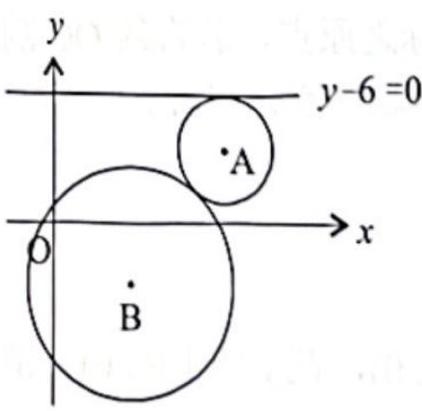
\includegraphics[max width=\textwidth]{2024_06_07_f484519cd4dc635602b3g-04}
% \end{center}

% [2009 年第 7(b)㓳]

% \begin{enumerate}[leftmargin=*]
%   \setcounter{enumi}{10}
%   \item 已知 $\mathrm{A}, \mathrm{B}$ 两点的坐标分别是 $(-1,0)$ 及 $(0,2)$ 。若 $\mathrm{P}$ 是圆 $x^{2}+y^{2}-2 x=0$ 上的任意点,求 $\triangle P A B$ 的面积的最大可能值。
% \end{enumerate}

% \section*{15.4] 四的切线}
% (选择䞨)

% \begin{enumerate}[leftmargin=*]
%   \item 求目 $x^{2}+y^{2}=50$, 在点 $(1,-7)$ 的切线方軖式.\\
% A $2 x+2 y=25$\\
% B $x-7 y=50$\\
% C $x+7 y=50$\\
% D $7 x+y=50$\\
% E $x+y=50$
% \end{enumerate}

% [1977 年第 14 顽]

% \begin{enumerate}[leftmargin=*]
%   \setcounter{enumi}{1}
%   \item 求自点 $(3,3)$ 至圆 $x^{2}+y^{2}-2 x+4 y+1=0$ 的切线的长。\\
% A 5\\
% B $\sqrt{17}$\\
% C 25\\
% D 10\\
% E $\sqrt{33}$
% \end{enumerate}

% [1977 年第 15 题]

% \begin{enumerate}[leftmargin=*]
%   \setcounter{enumi}{2}
%   \item 求自点 $(3,4)$ 至圆 $x^{2}+4 x-4 y+4=0$ 的切线长。\\
% A $\sqrt{29}$\\
% B 4\\
% C 5\\
% D 3\\
% E 2
% \end{enumerate}

% [1978 年第 15 题]

% \begin{enumerate}[leftmargin=*]
%   \setcounter{enumi}{3}
%   \item 若直线 $2 x+3 y+3 \sqrt{13}=0$ 与圆 $x^{2}+y^{2}=k$ 相切, 则 $k$ 之值为\begin{enumerate}[leftmargin=*] .\\
% A 0\\
% B 1\\
% C $3 \sqrt{3}$\\
% D 9\\
% E 以上皆非
% \end{enumerate}

% [1983 年第 14 题]

% \begin{enumerate}[leftmargin=*]
%   \setcounter{enumi}{4}
%   \item 从点 $\mathrm{A}(3,-4)$ 至圆 $x^{2}+y^{2}+6 x-8 y=0$ 所引切线, 其长等于\begin{enumerate}[leftmargin=*]\\
% A $2 \sqrt{2}$\\
% B $3 \sqrt{2}$\\
% C $5 \sqrt{3}$\\
% D $7 \sqrt{5}$\\
% E $9 \sqrt{7}$
% \end{enumerate}

% [1990 年第 15 题]

% \begin{enumerate}[leftmargin=*]
%   \setcounter{enumi}{5}
%   \item 若直线 $3 x-4 y=k$ 是圆 $x^{2}+y^{2}+2 x-4 y+1=0$ 的切线, 试求 $k$ 之值。\\
% A -1 或 -21\\
% B -1 或 21\\
% C 1 或 21\\
% D -21\\
% E -1
% \end{enumerate}

% [1991 年第 13 题]

% \begin{enumerate}[leftmargin=*]
%   \setcounter{enumi}{6}
%   \item 求从点 $(1,-2)$ 引圆 $(x-10)^{2}+(y-8)^{2}=15$ 的切线的长度。\\
% A 14\\
% B $\sqrt{142}$\\
% C $\sqrt{166}$\\
% D $2 \pi$\\
% E 以上皆非
% \end{enumerate}

% [1993 年第 13 题]

% \begin{enumerate}[leftmargin=*]
%   \setcounter{enumi}{7}
%   \item 求圆 $x^{2}+y^{2}=4$ 的切线的方程式, 它与圆的直径 $y=\frac{3}{4} x$ 平行。\\
% A $y=\frac{3}{4} x \pm \frac{5}{2}$\\
% B $y=\frac{3}{4} x \pm \frac{5}{4}$\\
% C $y=\frac{3}{4} x \pm 2$\\
% D $y=\frac{3}{4} x \pm 4$\\
% E 以上皆非
% \end{enumerate}

% [1995 年第 14 题]

% \begin{enumerate}[leftmargin=*]
%   \setcounter{enumi}{8}
%   \item 声搆轮 $y=-2 x+c$ 切约 $x^{2}+y^{2}-6 x+12 y+40=0$, 则 $c$ 的佰是\begin{enumerate}[leftmargin=*] -\\
% A $\pm \sqrt{2}$\\
% B $\pm \sqrt{3}$\\
% C $\pm 2$\\
% D $\pm \sqrt{5}$\\
% E $\pm 5$
% \end{enumerate}

% [1998 年第14 清

% \begin{enumerate}[leftmargin=*]
%   \setcounter{enumi}{9}
%   \item 从古 $\mathrm{A}(4, y)$ 向购 $(x+3)^{2}+(y-4)^{2}=5^{2}$ 引切线, 则切距的最小值是\begin{enumerate}[leftmargin=*] .\\
% A 4\\
% B $2 \sqrt{6}$\\
% C 6\\
% D 7\\
% E 24
% \end{enumerate}

% [2002 年第 15 倩

% \begin{enumerate}[leftmargin=*]
%   \setcounter{enumi}{10}
%   \item 如果直线 $y-2=k(x-1)$ 是圆 $x^{2}+y^{2}=1$ 的一条切线, 则此切线的方程式思\begin{enumerate}[leftmargin=*]\\
% A $3 x-4 y+5=0$\\
% B $3 x+4 y-5=0$\\
% C $3 x+4 y-11=0$\\
% D $3 x-4 y+5=0$ 或 $x-1=0$\\
% E $3 x+4 y-11=0$ 或 $x-1=0$
% \end{enumerate}

% [2003 年第 13 迡]

% \begin{enumerate}[leftmargin=*]
%   \setcounter{enumi}{11}
%   \item 两圆 $x^{2}+y^{2}+2 x-6 y-26=0$ 与 $x^{2}+y^{2}-4 x+2 y+4=0$ 有几条公切线?\\
% A 4\\
% B 3\\
% C 2\\
% D 1\\
% E 0
% \end{enumerate}

% [2006年第 9 题]

% \begin{enumerate}[leftmargin=*]
%   \setcounter{enumi}{12}
%   \item 直线 $7 x-24 y+8=0$ 是圆心为 $(2,3)$ 的圆的切线。求这个圆的半径。\\
% A 1\\
% B 2\\
% C 3\\
% D 5\\
% E 25
% \end{enumerate}

% [2008 年第 1 题]

% \begin{enumerate}[leftmargin=*]
%   \setcounter{enumi}{13}
%   \item 求圆 $x^{2}+y^{2}-6 x-4 y+4=0$ 上两条平行切线之间的距离。\\
% A 2\\
% B 3\\
% C 6\\
% D 9\\
% E 18
% \end{enumerate}

% [2009 年第 1 题]

% \begin{enumerate}[leftmargin=*]
%   \setcounter{enumi}{14}
%   \item 若从点 $(a, 1)$ 到圆 $x^{2}+y^{2}+5 x+7 y+3=0$ 的切线长是 5 , 求 $a$ 的值。\\
% A -7 或 -2\\
% B -7 或 2\\
% C -3 或 -2\\
% D -3 或 2\\
% E 3 或2
% \end{enumerate}

% [2011 年第 12 颌]

% \section*{(作答题)}
% \begin{enumerate}[leftmargin=*]
%   \item 直线 $\mathrm{AB}, \mathrm{AC}$ 分别切圆 $\mathrm{O}$ 于 $\mathrm{B}, \mathrm{C}$ 两点。求证 $\mathrm{AB}=\mathrm{AC}$ 。

%   \item 求切于 $x$ 轴及直线 $3 x-4 y+3=0$ 且约心在王线 $x+y=3$ 上的四之方罣式。

% \end{enumerate}

% [1978 年第 7 処]

% \begin{enumerate}[leftmargin=*]
%   \setcounter{enumi}{2}
%   \item 求自点 $\mathrm{P}(4,2)$ 作因 $x^{2}+y^{2}-4 x+4 y-2=0$ 之切线的方䙵式。
% \end{enumerate}

% [1984 年第 3(a)题]

% \begin{enumerate}[leftmargin=*]
%   \setcounter{enumi}{3}
%   \item 求由一定点 $(2,2)$ 至圆 $2 x^{2}+2 y^{2}+2 x+4 y-1=0$ 的切距。
% \end{enumerate}

% [1987 年第 5(b)题]

% \begin{enumerate}[leftmargin=*]
%   \setcounter{enumi}{4}
%   \item 两圆都与 $x, y$ 两轴相切且通过点 $\mathrm{A}(8,1)$ 。试求
% \end{enumerate}

% (i) 两圆的方程式:

% (ii) 两圆的另一交点之坐标;

% (iii) 在 $\mathrm{A}$ 点每一圆的切线之方程式。

% (iv) 在 $\mathrm{A}$ 点两切线所夹锐角。

% [1989 年第 6(a)题]

% \begin{enumerate}[leftmargin=*]
%   \setcounter{enumi}{5}
%   \item (a) 如果圆 $x^{2}+y^{2}+2 g x+2 f y+c=0$ 上一点 $\left(x_{0}, y_{0}\right)$ 所引切线与圆 $x^{2}+y^{2}=r^{2}$ 相切, 试证 $\left(g x_{0}+f y_{0}+c\right)^{2}=r^{2}\left(g^{2}+f^{2}-c\right)$ 。
% \end{enumerate}

% (b) 如果圆 $x^{2}+y^{2}-4 x-8 y-80=0$ 内的弦其长度及斜率分别为 $8 \sqrt{5}$ 及 $\frac{1}{2}$, 求这些弦的方程式。

% $[1990$ 年第 9 题]

% \begin{enumerate}[leftmargin=*]
%   \setcounter{enumi}{6}
%   \item 已知直线 $y=x+b$ 是圆 $x^{2}+y^{2}=4$ 的一条切线, 求 $b$ 的可能值。
% \end{enumerate}

% $[2000$ 年第 $7(b)$ 题 $]$

% \begin{enumerate}[leftmargin=*]
%   \setcounter{enumi}{7}
%   \item 在圆 $x^{2}+y^{2}=a^{2}$ 上一动点 $\mathrm{P}$ 的切线分别交座标轴 $\mathrm{OX}, \mathrm{OY}$ 于 $\mathrm{A}$ 和 $\mathrm{B}$, 且 $\mathrm{OAQB}$ 是一个长方形。试证明 $\mathrm{Q}$ 点的轨迹方程式是 $\frac{a^{2}}{x^{2}}+\frac{a^{2}}{y^{2}}=1$ 。
% \end{enumerate}

% [2002 年第 9 (c)题]

% \begin{enumerate}[leftmargin=*]
%   \setcounter{enumi}{8}
%   \item (a) 求经过圆 $x^{2}+y^{2}+2 x-4 y+1=0$ 与直线 $2 x-y+4=0$ 的交点且与 $y$ 轴相切的两圆的方程式。
% \end{enumerate}

% (b) 求过原点到此二圆所作的另两条切线的方程式。

% \begin{enumerate}[leftmargin=*]
%   \setcounter{enumi}{9}
%   \item 求 $x^{2}+y^{2}+4 x-10 y-7=0$ 的想心及半经。䁌此, 或其他方法, 若 $y=2 x+c$ 是此四的切线, 来 $c$ 的设。
% \end{enumerate}

% $(3 \%)$

% [2007 年第 7(a)廼]

% \begin{enumerate}[leftmargin=*]
%   \setcounter{enumi}{10}
%   \item 求两条由点 $(-2,3)$ 至目 $x^{2}+y^{2}+2 x-12 y+32=0$ 的切线方程式。
% \end{enumerate}

% [2010 年第 $7(b)$ 顷]

% \begin{enumerate}[leftmargin=*]
%   \setcounter{enumi}{11}
%   \item 求经过点 $\mathrm{M}(3,-4)$ 且与圆 $x^{2}+y^{2}+2 x-6 y+5=0$ 相切于点 $\mathrm{P}(1,2)$ 的圆的方程式。 $(6 \%)$ [2014 年第 $7(b)$ 輀 $]$
% \end{enumerate}

% \section*{[5.5] 两圆正切、正交}
% \section*{(选择题)}
% \begin{enumerate}[leftmargin=*]
%   \item 两圆 $x^{2}+y^{2}+3 x-2 y-20=0$ 及 $x^{2}+y^{2}-2 x+3 y-5=0$ 的公共弦的方程式是\\
% A $x+y-3=0$\\
% B $x-y-3=0$\\
% $x-y-5=0$\\
% D $2 x+y-3=0$\\
% E $\quad x-2 y+3=0$
% \end{enumerate}

% C

% [1987 年第 6 题]

% \begin{enumerate}[leftmargin=*]
%   \setcounter{enumi}{1}
%   \item 已知两圆 $x^{2}+y^{2}+k x-6 y+5=0$ 与 $x^{2}+y^{2}+2 x+y-1=0$ 正交(Cut orthogonally), $k$之值为\begin{enumerate}[leftmargin=*]。\\
% A -9\\
% B $\quad-7$\\
% C 5\\
% D 7\\
% E 9
% \end{enumerate}

% [1988 年第 19 题]

% \begin{enumerate}[leftmargin=*]
%   \setcounter{enumi}{2}
%   \item 如果两圆 $x^{2}+y^{2}=1$ 及 $x^{2}+y^{2}-6 x+a y+9=0$ 相切, 求 $a$ 的值。\\
% A $\pm 10$\\
% B $\pm 8$\\
% C $\pm 6$\\
% D $\pm 4$\\
% E 0
% \end{enumerate}

% [1992 年第 13 题]

% \begin{enumerate}[leftmargin=*]
%   \setcounter{enumi}{3}
%   \item 如果两圆 $x^{2}+y^{2}-4=0$ 及 $x^{2}+y^{2}+2 a x-6 y+a=0$ 正交(Cut orthogonally), 则常数 $a$的值等于\begin{enumerate}[leftmargin=*] -\\
% A 4\\
% B 3\\
% C 2\\
% D 1\\
% E 0
% \end{enumerate}

% [1992 年第 15 题]

% \begin{enumerate}[leftmargin=*]
%   \setcounter{enumi}{4}
%   \item 已知两圆 $(x-a)^{2}+(y-b)^{2}=c^{2}$ 与 $(x-b)^{2}+(y-a)^{2}=c^{2}$ 交于一点, 求 $a, b$ 及 $c$ 的关系。\\
% A $(a-b)^{2}=2 c^{2}$\\
% B $(a+b)^{2}=2 c^{2}$\\
% C $(a-b)^{2}=c^{2}$\\
% D $(a+b)^{2}=c^{2}$\\
% E 以上都不是

%   \item 若两圆 $x^{2}+y^{2}+6 x+10 y+c=0$ 与 $x^{2}+y^{2}+4 x-2 y+3=0$ 正交, 求 $c$ 的傎。\\
% A 3\\
% B 1\\
% C -1\\
% D $\quad-2$\\
% E -3

% \end{enumerate}

% [2012 年第 15 题]

% \begin{enumerate}[leftmargin=*]
%   \setcounter{enumi}{6}
%   \item 若两圆 $x^{2}+y^{2}-k x-2 y-52=0$ 与 $x^{2}+y^{2}+(2 k+1) x+8 y+26=0$ 正交, 求 $k$ 的值。\\
% A $-\frac{9}{2}$ 或 4\\
% B $-\frac{9}{2}$ 或 2\\
% C $\frac{9}{2}$ 或 -4\\
% D $\frac{9}{2}$ 或 -2\\
% E $\frac{9}{2}$ 或 2
% \end{enumerate}

% [2013 年第 15 题]

% \section*{(作答题)}
% \begin{enumerate}[leftmargin=*]
%   \item 二圆外切于 $\mathrm{A}$, 公切线 $\mathrm{PQ}$ 切二圆于 $\mathrm{P}, \mathrm{Q} ; \mathrm{RAS}$ 是一直线且再遇二圆于 $\mathrm{R}, \mathrm{S}$, 连 $\mathrm{RP}$, $S Q$ 并延长之使交于 $\mathrm{X}$ 。求证
% \end{enumerate}

% (a) $\triangle \mathrm{APQ} \sim \triangle \mathrm{XRS}$;

% (b) $P, A, Q, X$ 四点共圆。

% [1976 年第 9 题]

% \begin{enumerate}[leftmargin=*]
%   \setcounter{enumi}{1}
%   \item 已知 $a^{2}+b^{2}=c^{2}$, 试证两圆 $x^{2}+y^{2}+a x+b y=0$ 及 $x^{2}+y^{2}=c^{2}$ 相切, 并求其切点之座标。

%   \item (a) 若两圆 $x^{2}+y^{2}+2 g_{1} x+2 f_{1} y+c_{1}=0$ 与 $x^{2}+y^{2}+2 g_{2} x+2 f_{2} y+c_{2}=0$ 正交, 证明

% \end{enumerate}

% $$
% 2\left(g_{1} g_{2}+f_{1} f_{2}\right)=c_{1}+c_{2}
% $$

% (b) 若一直径的两端点为 $(0,4)$ 及 $(4,2)$ 的圆与另一圆 $x^{2}+y^{2}+2 k x-6 y+k=0$ 正交, 试应用(a)的结果或以其他方法求 $k$ 的值。

% (3\%)

% [1996 年第 $8(b)(c)$ 题]

% \begin{enumerate}[leftmargin=*]
%   \setcounter{enumi}{3}
%   \item 一圆的圆心落在第一象限上且与 $y$ 轴相切于点 $(0,3)$, 并与圆 $x^{2}+y^{2}-8 x+4 y-5=0$ 正交。求此圆的方程式。
% \end{enumerate}

% [2004 年第 7(a)题]

% \begin{enumerate}[leftmargin=*]
%   \setcounter{enumi}{4}
%   \item 如果一个动圆与圆 $x^{2}+y^{2}+2 g x+2 f y+c=0$ 正交, 且与 $x$ 轴相切。求这个动圆圆心的轨迹方程式。

%   \item 已知两败的方侑式为 $x^{2}+y^{2}+2 x-6 y=0$ 及 $x^{2}+y^{2}+3 x-5 y+6=0$ 。 证明其中一完全在乐一婴内。

% \end{enumerate}

% $(40$

% [2011 年第 8(b) 勘

% \begin{enumerate}[leftmargin=*]
%   \setcounter{enumi}{6}
%   \item 已知一团 $C$ 的半径为 3. 其罒心在䛖械 $x+y=1$ 上。若圆 $x^{2}+y^{2}=4$ 内切于圆 $C, y$ C的所有可恠方㱐式。
% \end{enumerate}

% (4)

% [2012 年第 9(a) 题


\end{document}